\documentclass{article}
\usepackage[compat=1.1.0]{tikz-feynman}
\usepackage{tikz}
\begin{document}

\begin{figure}
\centering
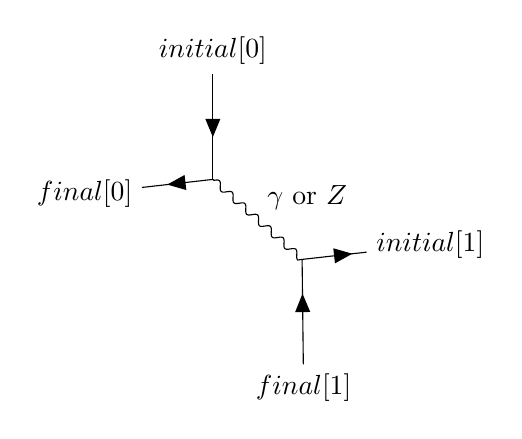
\begin{tikzpicture}
\begin{feynman}
\diagram{
    i1 [particle=\({{ initial[0] }}\)] -- [fermion] a -- [fermion] f1 [particle=\({{ final[0] }}\)],
    i2 [particle=\({{ initial[1] }}\)] -- [anti fermion] b -- [anti fermion] f2 [particle=\({{ final[1] }}\)],
    a -- [boson, edge label=\(\gamma\) or \(Z\)] b,
};
\end{feynman}
\end{tikzpicture}
\end{figure}

\end{document}